\documentclass[11pt]{article}

\usepackage[T1]{fontenc}
\usepackage{amsmath, amssymb, amsthm, mathtools}
\usepackage{listings}
\usepackage{xcolor}
\usepackage{geometry}
\usepackage{microtype}
\usepackage{booktabs}
\usepackage{longtable}
\usepackage{array}
\usepackage[inline]{enumitem}
\usepackage{stmaryrd}   % for \llbracket, \rrbracket
\usepackage[numbers,sort&compress]{natbib}
\usepackage{tikz}
\usetikzlibrary{arrows.meta,positioning,fit,calc}
\usepackage[hidelinks]{hyperref}

\geometry{margin=1in}
\let\origtextsc\textsc
\renewcommand{\textsc}[1]{\textup{\textmd{\origtextsc{#1}}}}
\setlength{\emergencystretch}{3em}

\newtheorem{theorem}{Theorem}[section]
\newtheorem{lemma}[theorem]{Lemma}
\newtheorem{corollary}[theorem]{Corollary}
\newtheorem{proposition}[theorem]{Proposition}
\theoremstyle{definition}
\newtheorem{definition}[theorem]{Definition}
\newtheorem{example}[theorem]{Example}
\newtheorem{remark}[theorem]{Remark}
\theoremstyle{remark}
\newtheorem*{notation}{Notation}

\definecolor{codegreen}{rgb}{0,0.6,0}
\definecolor{codegray}{rgb}{0.5,0.5,0.5}
\definecolor{codepurple}{rgb}{0.58,0,0.82}
\definecolor{backcolour}{rgb}{0.97,0.97,0.97}

\lstdefinelanguage{Rust}{
  keywords={fn, trait, struct, enum, impl, type, async, await, pub, let,
             mut, self, return, use, where, for, if, else, match, in,
             Option, Result, Box, Vec, bool},
  keywordstyle=\color{codepurple}\bfseries,
  ndkeywords={String, u64, usize},
  ndkeywordstyle=\color{codegreen},
  sensitive=true,
  comment=[l]{//},
  morecomment=[s]{/*}{*/},
  commentstyle=\color{codegray}\itshape,
  stringstyle=\color{codegreen},
  morestring=[b]",
}
\lstset{
  backgroundcolor=\color{backcolour},
  basicstyle=\ttfamily\small,
  breakatwhitespace=false,
  breaklines=true,
  captionpos=b,
  keepspaces=true,
  numbers=left,
  numbersep=5pt,
  numberstyle=\tiny\color{codegray},
  showspaces=false,
  showstringspaces=false,
  showtabs=false,
  tabsize=2,
  language=Rust,
}

\newcommand{\infrule}[3][]{%
  \resizebox{\ifdim\width>\linewidth \linewidth\else \width\fi}{!}{$\displaystyle
    \begin{array}{c}
      #2 \\[-2pt]
      \hline\\[-9pt]
      #3
    \end{array}%
    \ifx\relax#1\relax\else\;\;[\textsc{#1}]\fi$%
  }%
}
\newcommand{\fitwidth}[1]{%
  \resizebox{\ifdim\width>\linewidth \linewidth\else \width\fi}{!}{#1}}
\newcommand{\rulebox}[3][]{%
  \[
    \infrule[#1]{#2}{#3}
  \]
}

\newcommand{\Agent}{\ensuremath{\mathbf{Agent}}}
\newcommand{\Oracle}{\ensuremath{\mathbf{Oracle}}}
\newcommand{\Chan}{\ensuremath{\mathbf{Chan}}}
\newcommand{\Mem}{\ensuremath{\mathbf{Mem}}}
\newcommand{\Journal}{\ensuremath{\mathbf{Journal}}}
\newcommand{\Supervisor}{\ensuremath{\mathbf{Sup}}}
\newcommand{\step}{\;\leadsto\;}
\newcommand{\stepprob}[1]{\;\xrightarrow{#1}\;}
\newcommand{\conf}[4]{\langle #1,\, #2,\, #3,\, #4 \rangle}
\newcommand{\prob}[1]{\Pr\!\left[#1\right]}
\newcommand{\expect}[1]{\mathbb{E}\!\left[#1\right]}
\newcommand{\dist}{\mu}
\newcommand{\record}{\textsc{rec}}
\newcommand{\replay}{\textsc{rep}}
\newcommand{\fault}{\,\lightning}
\newcommand{\obsleq}{\sqsubseteq_{\mathrm{obs}}}
\newcommand{\journal}{\mathcal{J}}
\providecommand{\sched}{\mathfrak{s}}
\newcommand{\fullconf}[5]{\langle #1;\, #2;\, #3;\, #4;\, #5 \rangle}
\newcommand{\stepm}[1]{\;\xrightarrow{}\;_{\!\!#1}\;}
\newcommand{\Dirac}[1]{\delta_{#1}}
\newcommand{\OD}[3]{\mathsf{OracleDraw}(#1,#2,#3)}
\newcommand{\CR}[2]{\mathsf{ChannelRecv}(#1,#2)}
\newcommand{\Eff}[4]{\mathsf{Effect}(#1,#2,#3,#4)}
\newcommand{\key}{\mathsf{key}}
\newcommand{\lookup}{\mathsf{lookup}}
\newcommand{\Low}{\mathit{Lo}}
\newcommand{\obs}{\mathrm{obs}}
\newcommand{\erase}[1]{\lfloor #1 \rfloor_{\Low}}
\newcommand{\Sched}{\mathfrak{S}}
\newcommand{\Prob}[2]{\mathbb{P}_{#1,#2}}
\newcommand{\meas}[1]{\mu_{#1}}

% Notation macros (see Appendix A)
\newcommand{\labelLat}{\mathcal{L}}
\newcommand{\labelLeq}{\sqsubseteq}
\newcommand{\labelJoin}{\sqcup}
\newcommand{\labLow}{\mathsf{Low}}
\newcommand{\labHigh}{\mathsf{High}}
\newcommand{\Dist}{\mathcal{D}}
\newcommand{\Jour}{J}
\newcommand{\jappend}[2]{#1 \cdot #2}
\newcommand{\ClockEv}[2]{\mathsf{Clock}(#1,#2)}
\newcommand{\JKSort}{\mathcal{K}}
\newcommand{\jproj}[2]{#1 \upharpoonright #2}
\newcommand{\Cursor}{\mathsf{Cursor}}
\newcommand{\WL}[2]{\mathsf{WL}(#1,#2)}
\newcommand{\schedLo}{\mathfrak{s}^{\Low}}
\newcommand{\scong}{\equiv}
\newcommand{\traceq}{\approx}
\newcommand{\bigstep}{\Downarrow}
\newcommand{\labTau}{\tau}
\newcommand{\labOracle}[1]{o(#1)}
\newcommand{\labSend}[2]{#1\,!\,#2}
\newcommand{\labRecv}[2]{#1\,?\,#2}
\newcommand{\labRead}[2]{\iota(#1,#2)}
\newcommand{\labWrite}[2]{\omega(#1,#2)}
\newcommand{\labEff}[2]{\mathsf{eff}(#1,#2)}
\newcommand{\labSpawn}[1]{\mathsf{spw}(#1)}
\newcommand{\labFault}{\,\lightning}
\newcommand{\schedhat}{\hat{\mathfrak{s}}}
\newcommand{\CouplingSpace}{\Omega}
\newcommand{\obsLo}[1]{\obs_{\Low}(#1)}
\newcommand{\lowEq}[1]{=_{\Low}}
\newcommand{\contract}[2]{\models_{#1} #2}
\newcommand{\decRestart}{\mathsf{restart}}
\newcommand{\decComp}[1]{\mathsf{compensate}(#1)}
\newcommand{\decEsc}{\mathsf{escalate}}
\newcommand{\decStop}{\mathsf{stop}}
\newcommand{\replayTerm}[2]{\mathsf{replay}(#1,\,#2)}
\newcommand{\Atag}[1]{(\mathrm{A}_{#1})}
\newcommand{\Qtag}[1]{\textbf{Q-#1}}

\title{%
  Provably Sound Replay and Crash Recovery \\
  for Nondeterministic LLM Agents
}

\author{
  Aniketh Bandlamudi \\
  \small University of Virginia \\
  \small\texttt{zpq3uh@virginia.edu}\quad\texttt{me@aniketh.net}
}

\date{November 2026}

\begin{document}

\maketitle

\begin{abstract}

Agents built on large language models (LLMs) run for minutes or hours, call tools with real
side effects, and crash.
Because model calls are nondeterministic, re-running a crashed agent re-samples every call
and can repeat work that already happened.
Durable-execution engines avoid this by recording each nondeterministic result and replaying
it, but they treat each result as an opaque value and say nothing about the distribution it
came from.
We give a small probabilistic semantics for an LLM agent in which every model call is a draw
from an abstract probability measure and every response is recorded in an append-only
journal, with record, replay, and resume modes.
We prove that replaying a run from its journal reproduces its trace and journal exactly, so
replay succeeds with probability~1 and record and replay induce the same distribution over
traces.
We also prove that after a crash at any point, resuming with fresh randomness behaves exactly
like an uninterrupted run whose randomness is spliced at the crash point, so the continuation
follows the original distribution conditioned on what survived, provided the crash does not
depend on a response that was never journaled.
The pointwise core of both results is mechanized in Lean~4 for every program tree and every
randomness tape; the probabilistic statements follow on paper.
Both results extend to systems of concurrently running agents that share memory and exchange
messages, under any deterministic scheduler and with a single global journal, by a reduction
to the single-agent case; the generic lifting is mechanized, and its instantiation to the
multi-agent calculus is on paper.
For such systems we prove a probabilistic noninterference theorem: under a floating-label
discipline and a priority scheduler whose priorities depend only on public events, an agent's
secret data does not influence, even statistically, what public observers see.
A dependency-free Rust prototype implements the semantics, together with write-ahead logging
for tool side effects.
On it, 1,000 of 1,000 replays reproduce their run, and recovery from all 4,664 crash points
tested completes without repeating a committed side effect.
Journal appends take about 100 nanoseconds.
We state precisely which restrictions these guarantees need and what lifting them requires.

\end{abstract}

\tableofcontents
\newpage

\section{Introduction}

\subsection*{The problem}

Large language models are increasingly deployed as autonomous agents that plan, call tools,
and keep long-running state.
Such runs fail often~\citep{cemri2025mast}, and they are hard to make durable.
A run may last minutes or hours and call external tools with real side effects, and when the
process crashes part-way through, the obvious recovery, re-running the agent from the start,
re-samples every model call.
The new run may take a different path, and it may repeat side effects that already happened.

Durable-execution engines, exemplified by Temporal~\citep{temporal2024docs}, solve the
engineering half of this problem by recording an event history.
Workflow code must be deterministic; calls to the outside world, including LLM calls, run as
\emph{Activities} whose results are recorded once and returned from the history on replay.
The idea is classical: logging every nondeterministic event so that a piecewise-deterministic
process can be replayed after a failure is the basis of message-logging recovery in
distributed systems~\citep{strom1985optimistic,elnozahy2002survey}.
For an LLM agent, however, this treats each model call as an opaque recorded value.
The engine makes replay correct but gives no account of the distribution the value was drawn
from, so it cannot say whether replay preserves the probability of a run, or what the
distribution of the rest of a run is after recovery.
Recent tools for LLM agents record and replay runs at their nondeterministic
boundaries~\citep{mudasiru2026agrepl,chawla2026chronicle} and check resume behaviour against
machine-checked contracts~\citep{khan2026resume,zheng2026execedits}, but they too are
deterministic or empirical.

Formal models of LLM agents, meanwhile, have focused elsewhere.
LLMbda~\citep{garby2026llmbda} gives a probabilistic, Lean-verified semantics for a single
agent's program with information-flow control, and $\lambda_A$~\citep{liu2026lambdaA} and
PPDL~\citep{mandel2026ppdl} give probabilistic semantics to agent programs and LLM flows.
The MSC calculus~\citep{bollig2026msc} proves coordination properties of many agents while
treating model outputs as arbitrary.
None of them models journaling, replay, or crash recovery.

\subsection*{Contribution}

We give a minimal probabilistic semantics for durable replay of an LLM agent and prove that
replay and crash recovery are sound in a precise probabilistic sense.

\begin{enumerate}

\item \textbf{A probabilistic semantics with a journal (Section~\ref{sec:semantics}).}
Every model call is a draw from an abstract probability measure and every response is recorded
in an append-only journal; the agent runs in record, replay, or resume mode.
Fixing the randomness on a tape lets runs in different modes be compared directly.

\item \textbf{Replay soundness (Theorem~\ref{thm:replay}).}
Replaying a run from its journal reproduces its trace and journal exactly.
Replay therefore succeeds with probability~1, and recording then replaying induces the same
distribution over traces as recording alone.

\item \textbf{Crash recovery (Corollary~\ref{cor:resume}).}
After a crash at any point, resuming with fresh randomness behaves exactly like an
uninterrupted run whose randomness is spliced at the crash point.
Resuming with the same randomness reproduces the original run, and resuming with fresh
randomness continues it with the original distribution conditioned on what survived, provided
the crash does not depend on a response that was never journaled.

\item \textbf{Many agents (Section~\ref{sec:multiagent}).}
Under any deterministic scheduler and with a single global journal, a system of concurrently
running agents that share memory and exchange messages unfolds into a single program tree, so
replay soundness and crash recovery carry over to whole systems (Theorem~\ref{thm:sys}).
We also prove a noninterference theorem for concurrently scheduled agents
(Theorem~\ref{thm:ni}): under a floating-label discipline, with labels on memory cells and
channels that never change, and a priority scheduler whose priorities depend only on public
events, the public trace of a system is the same whatever its secret data, pointwise for every
family of per-agent randomness tapes and hence in distribution.

\item \textbf{A Lean mechanization (Section~\ref{sec:mechanization}).}
The pointwise core of both results, and their generic lifting to any deterministic step
system, are proved in Lean~4 for every program tree, randomness tape, starting cursor, and
crash point, with no unproven steps; the instantiation to the multi-agent calculus and
the noninterference theorem are proved on paper.

\item \textbf{A prototype and measurements (Sections~\ref{sec:rust-runtime}
and~\ref{sec:evaluation}).}
A dependency-free Rust crate implements the semantics together with write-ahead logging for
tool side effects.
We measure replay determinism, recovery from a crash at every journal position, and journaling
overhead.

\end{enumerate}

\noindent
The paper's source, the Lean development, and the Rust prototype with all experiment
harnesses are available at \url{https://github.com/ankthba/agentical}.

\subsection*{Scope}

Logging nondeterministic events for replay is not new; what is new is a semantics in which
recovery with fresh randomness provably preserves the distribution of a run
(Corollary~\ref{cor:resume}(ii)), not only individual runs.
Replay never repeats a side effect, but whether recovery may perform an interrupted effect
again depends on the external world, which we do not formalize (Section~\ref{sec:effects}).
The multi-agent results assume deterministic scheduling and a single global journal; the
prototype runs a single agent. Section~\ref{sec:limitations} lists what lifting these
restrictions requires.

\subsection*{Roadmap}

Section~\ref{sec:background} reviews probabilistic semantics and durable execution.
Section~\ref{sec:semantics} defines the calculus, Section~\ref{sec:metatheory} proves replay
soundness and crash recovery, and Section~\ref{sec:multiagent} extends both to systems of
agents and proves noninterference.
Section~\ref{sec:rust-runtime} describes the prototype and Section~\ref{sec:evaluation} the
experiments.
Section~\ref{sec:related} discusses related work, Section~\ref{sec:limitations} limitations and
future work, and Section~\ref{sec:conclusion} concludes.


\section{Background}
\label{sec:background}

This section reviews the two traditions the paper connects: probabilistic semantics, and
durable execution by logging and replay.

\subsection{Probabilistic Semantics}
\label{sec:bg-prob}

Probabilistic program semantics goes back at least to Kozen~\citep{kozen1981semantics}, who
interpreted programs as transformers of probability measures.
Borgstr\"{o}m et al.~\citep{borgstrom2016probabilistic} give distribution-based big-step and
small-step semantics for a probabilistic call-by-value $\lambda$-calculus and prove them
equivalent, together with a sampling-based semantics that agrees with them when integrated over
traces.
Our semantics is of the sampling kind: a run reads its random choices from a tape, and the
distribution over runs is induced by the distribution over tapes (Lemma~\ref{lem:tape}).
Fixing the tape is also what lets us compare runs in different modes directly, an instance of
the coupling method for relational reasoning about probabilistic
programs~\citep{barthe2015coupling}.
Probabilistic automata~\citep{segala1995probabilistic} add nondeterministic choice, resolved by
a scheduler, to probabilistic transitions; a single agent needs no scheduler, but concurrent
agents would (Section~\ref{sec:limitations}).

\subsection{Durable Execution}
\label{sec:bg-durable}

Durable-execution systems, Temporal~\citep{temporal2024docs} being the canonical production
example, give long-running workflows crash-recoverable semantics.
The mechanism is an \emph{event history}: an append-only log of all externally determined
values received by the workflow.
On restart, the workflow code is re-executed from the beginning, but any call that would
normally block on an external response instead returns the stored value from the log.
Workflow code must therefore be deterministic: re-run against the same history, it must make
the same decisions.
Calls to the outside world, including LLM calls, run as \emph{Activities} whose results are
recorded once and thereafter returned from the history, and other nondeterministic values such
as random numbers are obtained through replay-safe SDK operations that record
them~\citep{temporal2026sideeffects}.
This makes replay correct, but it gives no semantics to the \emph{distribution} of an
Activity's outcome, only to the single realized value.

The technique itself is classical.
Message-logging protocols for rollback recovery~\citep{strom1985optimistic,elnozahy2002survey}
assume that processes are \emph{piecewise deterministic}: execution is deterministic between
nondeterministic events, which are logged and replayed.
Our journal applies the same idea to an LLM agent, for which every model call is a
nondeterministic event, and our contribution is to state and prove its soundness inside a
probabilistic semantics.

\subsection{Comparison}

Table~\ref{tab:comparison} compares this work with the closest related systems;
Section~\ref{sec:related} discusses them in detail.

\begin{table}[ht]
\centering
\caption{Comparison with the closest related systems.
  \checkmark~= supported, $\times$~= not supported, $\sim$~= partial.}
\label{tab:comparison}
\fitwidth{%
\begin{tabular}{lccccc}
\toprule
\textbf{System} & \textbf{Multi-agent} & \textbf{Prob.\ semantics} & \textbf{Durable replay} & \textbf{Mechanized} & \textbf{Impl.} \\
\midrule
LLMbda~\citep{garby2026llmbda}
  & $\times$ & \checkmark & $\times$ & \checkmark{} (Lean) & \checkmark{} (verified interpreter) \\
MSC coord.~\citep{bollig2026msc}
  & \checkmark & $\times$ (black box) & $\sim$ (ZipperGen, informal) & \checkmark{} (Lean~4) & \checkmark{} (Python) \\
Temporal~\citep{temporal2024docs}
  & $\sim$ & $\times$ (det.\ required) & \checkmark & $\times$ & \checkmark \\
\textbf{This work}
  & $\times$ & \checkmark & \checkmark & \checkmark{} (Lean, pointwise) & \checkmark{} (Rust) \\
\bottomrule
\end{tabular}%
}
\end{table}


\section{A Probabilistic Semantics with a Journal}
\label{sec:semantics}

We give a small calculus for a single agent whose only source of nondeterminism is calls to
a language model, together with a journal that records every outcome.
The calculus is deliberately minimal: it isolates the part of an agent that durable
execution has to get right, namely the interplay between stochastic model calls and the
record that makes them reproducible.

\subsection{Syntax}
\label{sec:syntax}

Let $\mathit{Val}$ be a countable set of values; prompts and model outputs are values (for
example, finite token sequences).
Expressions $e$ are pure and deterministic: $e \Downarrow v$ is a total function from closed
expressions to values, and we assume programs are well typed, so the condition of an
$\mathbf{if}$ evaluates to a boolean.
Terms are
\[
  M, N \;::=\; \mathbf{return}\;e
    \;\mid\; \mathbf{let}\;x = e\;\mathbf{in}\;M
    \;\mid\; \mathbf{if}\;e\;\mathbf{then}\;M\;\mathbf{else}\;N
    \;\mid\; \mathbf{let}\;x \Leftarrow \mathbf{oracle}(e)\;\mathbf{in}\;M .
\]
The term $\mathbf{let}\;x \Leftarrow \mathbf{oracle}(e)\;\mathbf{in}\;M$ asks the model with
the prompt that $e$ evaluates to and binds the response to $x$ in $M$.
An \emph{oracle} assigns to each prompt $p$ a probability measure $\meas{p}$ on
$\mathit{Val}$; since $\mathit{Val}$ is countable, $\meas{p}$ is discrete.
Nothing else is assumed about $\meas{p}$: the results below hold for every oracle.
The same construct models any externally determined value, such as a tool response, a
message from the environment, or a clock read; we speak of model calls for concreteness.
We omit general recursion, so every run makes finitely many oracle calls
(Section~\ref{sec:limitations} discusses lifting this).

\paragraph{Programs as trees.}
Because expressions are pure, the behaviour of a closed term is captured by its tree of
oracle calls: either it halts with a value, or it makes a call with some prompt $p$ and
continues with a subtree that depends on the response.
Formally, define $T(M)$ by
\begin{align*}
  T(\mathbf{return}\;e) &= \mathsf{halt}(v) && \text{where } e \Downarrow v,\\
  T(\mathbf{let}\;x = e\;\mathbf{in}\;M) &= T(M[v/x]) && \text{where } e \Downarrow v,\\
  T(\mathbf{if}\;e\;\mathbf{then}\;M\;\mathbf{else}\;N) &= T(M) \text{ or } T(N) && \text{as } e \Downarrow \mathsf{true} \text{ or } \mathsf{false},\\
  T(\mathbf{let}\;x \Leftarrow \mathbf{oracle}(e)\;\mathbf{in}\;M) &= \mathsf{draw}\bigl(p,\; v \mapsto T(M[v/x])\bigr) && \text{where } e \Downarrow p.
\end{align*}
Trees are well founded because terms have no recursion.
All definitions and results below depend only on $T(M)$, and the Lean development
(Section~\ref{sec:mechanization}) works directly with these trees.

\subsection{The Journal and Three Modes}
\label{sec:modes}

A \emph{journal} $J$ is a finite list of entries $(c, p, v)$: the cursor $c$ (the entry's
position in the log), the prompt $p$, and the response $v$.
The agent runs in one of three modes.
\begin{description}[noitemsep]
  \item[Record.] Each call is answered by the oracle, and its entry is appended to the journal.
  \item[Replay.] Each call is answered from the next journal entry; the oracle is not consulted.
  \item[Resume.] Replay until the journal is exhausted, then switch to record mode for the rest
    of the run. This is recovery after a crash.
\end{description}
A run emits a \emph{trace}: one label $o(c, p, v)$ per call, recording its cursor, prompt,
and response, followed by $\mathsf{done}(v)$ when the run halts with $v$.

\paragraph{Randomness tapes.}
To compare runs in different modes we fix their randomness in advance.
A \emph{tape} is a function $\omega : \mathbb{N} \times \mathit{Val} \to \mathit{Val}$, where
$\omega(c, p)$ is the response the oracle gives to prompt $p$ at cursor $c$.
Let $\Omega$ be the set of tapes with the product measure
$\mathbb{P} = \bigotimes_{(c,p)} \meas{p}$, under which the coordinates are independent and
$\omega(c,p)$ has law $\meas{p}$.
Since $\mathit{Val}$ is countable, so is the set of finite traces, so every set of traces is
measurable and every function of a run defined below is a random variable.

\paragraph{Semantics.}
Write $\mathsf{rec}(T, \omega, c)$, $\mathsf{rep}(T, J)$, and $\mathsf{res}(T, J, \omega, c)$
for the (trace, journal) pair produced by running tree $T$ from cursor $c$ in each mode:
\begin{align*}
  \mathsf{rec}(\mathsf{halt}(v), \omega, c) &= (\mathsf{done}(v),\; \varepsilon)\\
  \mathsf{rec}(\mathsf{draw}(p, k), \omega, c) &= o(c,p,v) \cdot \mathsf{rec}(k(v), \omega, c{+}1)
    && v = \omega(c,p), \text{ entry } (c,p,v)\\[3pt]
  \mathsf{rep}(\mathsf{halt}(v), J) &= (\mathsf{done}(v),\; \varepsilon)\\
  \mathsf{rep}(\mathsf{draw}(p, k), (c',p',v) \cdot J) &= o(c',p,v) \cdot \mathsf{rep}(k(v), J)
    && \text{entry } (c',p,v)\\
  \mathsf{rep}(\mathsf{draw}(p, k), \varepsilon) &= (\varepsilon, \varepsilon)
    && \text{journal exhausted}
\end{align*}
Here $\ell \cdot (t, J)$ prepends the label $\ell$ to the trace $t$ and the indicated entry to
$J$; replay re-emits each journal entry it consumes, so its output journal can be compared
with the recorded one.
Resume mode replays while the journal lasts and then records, tracking the cursor $c$ so that
the first fresh call lands at the position after the last surviving entry:
\begin{align*}
  \mathsf{res}(\mathsf{halt}(v), J, \omega, c) &= (\mathsf{done}(v),\; \varepsilon)\\
  \mathsf{res}(\mathsf{draw}(p, k), (c',p',v) \cdot J, \omega, c) &= o(c',p,v) \cdot \mathsf{res}(k(v), J, \omega, c{+}1)
    && \text{entry } (c',p,v)\\
  \mathsf{res}(\mathsf{draw}(p, k), \varepsilon, \omega, c) &= o(c,p,v) \cdot \mathsf{res}(k(v), \varepsilon, \omega, c{+}1)
    && v = \omega(c,p), \text{ entry } (c,p,v)
\end{align*}
These functions correspond to the small-step rules
\begin{align*}
  &\textsc{[O-rec]} && \langle \mathsf{draw}(p,k), J, c \rangle \xrightarrow{o(c,p,v)} \langle k(v), J\cdot(c,p,v), c{+}1 \rangle
     && \text{with probability } \meas{p}(\{v\}),\\
  &\textsc{[O-rep]} && \langle \mathsf{draw}(p,k), (c',p',v)\cdot R, c \rangle \xrightarrow{o(c',p,v)} \langle k(v), R, c{+}1 \rangle
     && \text{with probability } 1,\\
  &\textsc{[O-resume]} && \langle \mathsf{draw}(p,k), \varepsilon, c \rangle \text{ in resume mode steps as \textsc{[O-rec]}},
\end{align*}
where in replay and resume mode $R$ is the part of the journal not yet replayed.
In replay mode an exhausted journal at a call is stuck; in resume mode it falls through to
recording.
\textsc{[O-rec]} is the only rule whose successor is not a single configuration, so all
randomness in a run comes from oracle calls.
Replay checks neither the journaled prompt nor the cursor against the program: it trusts that
it is replaying the same program from the same starting cursor (assumption A2 below).

\begin{figure}[t]
  \centering
  \fitwidth{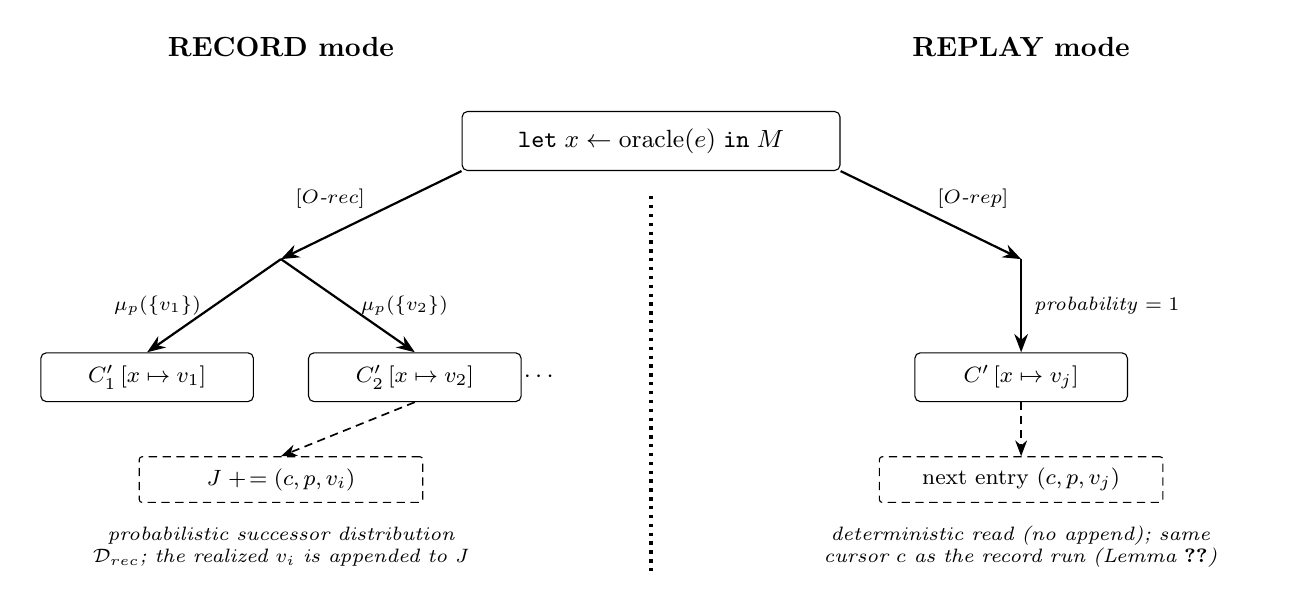
\begin{tikzpicture}[
  >=Stealth,
  every node/.style={align=center, font=\small},
  term/.style={draw, rounded corners=2pt, minimum width=4.8cm, minimum height=0.75cm, inner sep=3pt},
  state/.style={draw, rounded corners=2pt, minimum width=2.7cm, minimum height=0.62cm, inner sep=2pt, font=\footnotesize},
  jbox/.style={draw, densely dashed, rounded corners=1pt, minimum width=3.6cm, minimum height=0.58cm, inner sep=3pt, font=\footnotesize},
  lbl/.style={font=\scriptsize\itshape},
  arrow/.style={->, thick},
  darrow/.style={->, semithick, densely dashed},
]
\def\xR{-4.7}\def\xP{4.7}

\node[term] (draw) at (0,0) {$\texttt{let}\;x \leftarrow \mathrm{oracle}(e)\;\texttt{in}\;M$};
\node[font=\bfseries] at (\xR,1.2) {RECORD mode};
\node[font=\bfseries] at (\xP,1.2) {REPLAY mode};
\draw[very thick, dotted] (0,-0.7) -- (0,-5.5);

\coordinate (rb) at (\xR,-1.5);
\draw[arrow] (draw.south west) -- node[lbl, above left=-2pt]{$[O\text{-}rec]$} (rb);
\node[state] (v1) at (\xR-1.7,-3.0) {$C'_1\,[x\mapsto v_1]$};
\node[state] (v2) at (\xR+1.7,-3.0) {$C'_2\,[x\mapsto v_2]$};
\node at (\xR+3.3,-3.0) {$\cdots$};
\draw[arrow] (rb) -- node[lbl, left=1pt]{$\mu_p(\{v_1\})$} (v1.north);
\draw[arrow] (rb) -- node[lbl, right=1pt]{$\mu_p(\{v_2\})$} (v2.north);
\node[jbox] (jrec) at (\xR,-4.3) {$J \mathrel{+\!=} (c, p, v_i)$};
\draw[darrow] (v2.south) -- (jrec.north);
\node[lbl, text width=6.2cm] at (\xR,-5.15)
  {probabilistic successor distribution $\mathcal{D}_{rec}$; the realized $v_i$ is appended to $J$};

\coordinate (pb) at (\xP,-1.5);
\draw[arrow] (draw.south east) -- node[lbl, above right=-2pt]{$[O\text{-}rep]$} (pb);
\node[state] (vr) at (\xP,-3.0) {$C'\,[x\mapsto v_j]$};
\draw[arrow] (pb) -- node[lbl, right=1pt]{probability $=1$} (vr.north);
\node[jbox] (jrep) at (\xP,-4.3) {next entry $(c, p, v_j)$};
\draw[darrow] (vr.south) -- (jrep.north);
\node[lbl, text width=6.2cm] at (\xP,-5.15)
  {deterministic read (no append); same cursor $c$ as the record run (Lemma~\ref{lem:cursors})};
\end{tikzpicture}
}
  \caption{Record and replay of one oracle call.
    In record mode (left) the call samples $v \sim \meas{p}$ and appends $(c, p, v)$ to the
    journal. In replay mode (right) the same call reads the next entry with probability~1 and
    appends nothing new. The cursor $c$ does not depend on any sampled value
    (Lemma~\ref{lem:cursors}), so both modes address the same entry.}
  \label{fig:record-replay}
\end{figure}

\paragraph{The record distribution.}
The record run samples each response from the oracle as it goes.
Its distribution is that of $\mathsf{rec}(T, \omega, c)$ for $\omega \sim \mathbb{P}$:

\begin{lemma}[Tapes realize sampling]
\label{lem:tape}
Call $t = o(c,p_1,v_1) \cdots o(c{+}n{-}1,p_n,v_n)\,\mathsf{done}(v)$ a \emph{trace of $T$
from $c$} if it follows a path of $T$: each $p_i$ is the prompt $T$ issues after the responses
$v_1, \ldots, v_{i-1}$, and $T$ then halts with $v$.
For every tree $T$, cursor $c$, and finite trace $t$ of this form,
\[
  \mathbb{P}\bigl[\,\mathsf{rec}(T,\omega,c) \text{ has trace } t\,\bigr]
  \;=\; \prod_{i=1}^{n} \meas{p_i}(\{v_i\})
\]
if $t$ is a trace of $T$, and $0$ otherwise. This is the probability that the sampling
semantics (rule \textsc{[O-rec]}) produces $t$.
\end{lemma}

\begin{proof}
The $i$-th call of the run is made at cursor $c+i-1$ with a prompt $p_i$ that is determined by
the responses $v_1, \ldots, v_{i-1}$, and its response is the coordinate
$\omega(c+i-1, p_i)$.
The event that the run produces $t$ is therefore the event that
$\omega(c+i-1, p_i) = v_i$ for $i = 1, \ldots, n$, where $p_1, \ldots, p_n$ are the prompts
that $T$ issues along $t$ (fixed once $t$ is fixed).
These are $n$ distinct coordinates of the tape, so by independence the event has probability
$\prod_i \meas{p_i}(\{v_i\})$.
The sampling semantics produces $t$ with the same probability, by the chain rule:
given the first $i-1$ responses, the $i$-th is drawn from $\meas{p_i}$.
\end{proof}


\section{Replay Soundness and Crash Recovery}
\label{sec:metatheory}

We state three results: the cursors of a run do not depend on its randomness
(Lemma~\ref{lem:cursors}), replay reproduces a recorded run exactly
(Theorem~\ref{thm:replay}), and resuming after a crash continues the run with the
correct distribution (Corollary~\ref{cor:resume}).
Each comes in a pointwise form, quantified over every tree and every tape, which is
mechanized in Lean~4 (Section~\ref{sec:mechanization}), and a probabilistic form, which
follows on paper from the pointwise one.
Throughout we assume:
\begin{description}[noitemsep]
  \item[(A1)] $\mathit{Val}$ is countable and each $\meas{p}$ is a probability measure on it.
  \item[(A2)] Replay and resume run the same program, from the same starting cursor, as the
    recorded run.
  \item[(A3)] The journal is not corrupted or reordered; a crash keeps a prefix of it.
\end{description}

\begin{lemma}[Cursors]
\label{lem:cursors}
For every tree $T$, tape $\omega$, and cursor $c$, the $i$-th entry of the journal of
$\mathsf{rec}(T, \omega, c)$ has cursor $c+i-1$, whatever the responses (only the number of
entries depends on them).
\end{lemma}

\begin{proof}
By induction on $T$: each call appends one entry at the current cursor and advances it by one.
\end{proof}

\begin{theorem}[Replay soundness]
\label{thm:replay}
For every tree $T$, tape $\omega$, and cursor $c$, let $(t, J) = \mathsf{rec}(T, \omega, c)$.
Then
\[
  \mathsf{rep}(T, J) \;=\; (t, J).
\]
Consequently:
\begin{enumerate}[label=(\roman*), noitemsep]
  \item \textbf{(Trace equivalence)} replaying the journal reproduces the recorded trace,
    including every cursor, prompt, and response, and the journal itself;
  \item \textbf{(Determinism)} replay is a function of the journal alone and reads no
    randomness, so given $J$ it produces $t$ with probability~1;
  \item \textbf{(Equiprobability)} for every set $\Phi$ of traces,
    \[
      \mathbb{P}\bigl[\,\mathsf{rec}(T,\omega,c) \text{ has trace in } \Phi\,\bigr]
      \;=\;
      \mathbb{P}\bigl[\,\mathsf{rep}(T, J_\omega) \text{ has trace in } \Phi\,\bigr],
    \]
    where $J_\omega$ is the journal of $\mathsf{rec}(T,\omega,c)$; that is, recording and then
    replaying induces the same distribution over traces as recording alone, and by
    Lemma~\ref{lem:tape} a trace $o(c,p_1,v_1)\cdots o(c{+}n{-}1,p_n,v_n)\,\mathsf{done}(v)$
    of $T$ has probability $\prod_i \meas{p_i}(\{v_i\})$ under both.
\end{enumerate}
\end{theorem}

\begin{proof}
The identity is proved by induction on $T$.
For $\mathsf{halt}(v)$ both sides are $(\mathsf{done}(v), \varepsilon)$.
For $\mathsf{draw}(p, k)$, recording at cursor $c$ produces the entry $(c, p, v)$ with
$v = \omega(c,p)$ and continues as $\mathsf{rec}(k(v), \omega, c+1) = (t', J')$, so
$(t, J) = (o(c,p,v)\,t',\; (c,p,v)\,J')$.
Replay reads the entry $(c, p, v)$, emits $o(c, p, v)$, and continues as
$\mathsf{rep}(k(v), J')$, which equals $(t', J')$ by the induction hypothesis for the subtree
$k(v)$.
Part~(i) is the first component of the identity, and part~(ii) holds because $\mathsf{rep}$
does not take a tape.
For part~(iii), the identity holds for every $\omega$, so the two events are the same subset
of $\Omega$ and have the same probability; the product formula is Lemma~\ref{lem:tape}.
\end{proof}

\noindent
Part~(iii) is immediate from part~(i): it holds for every law on tapes, not only $\mathbb{P}$,
and the same is true of deterministic replay under any input distribution.
The probabilistic content of the paper lies elsewhere: in Lemma~\ref{lem:tape}, which says that
the tape semantics realizes sampling from the oracle, and in Corollary~\ref{cor:resume}(ii),
which says that recovery with fresh randomness preserves the distribution of a run.

\begin{figure}[t]
  \centering
  \fitwidth{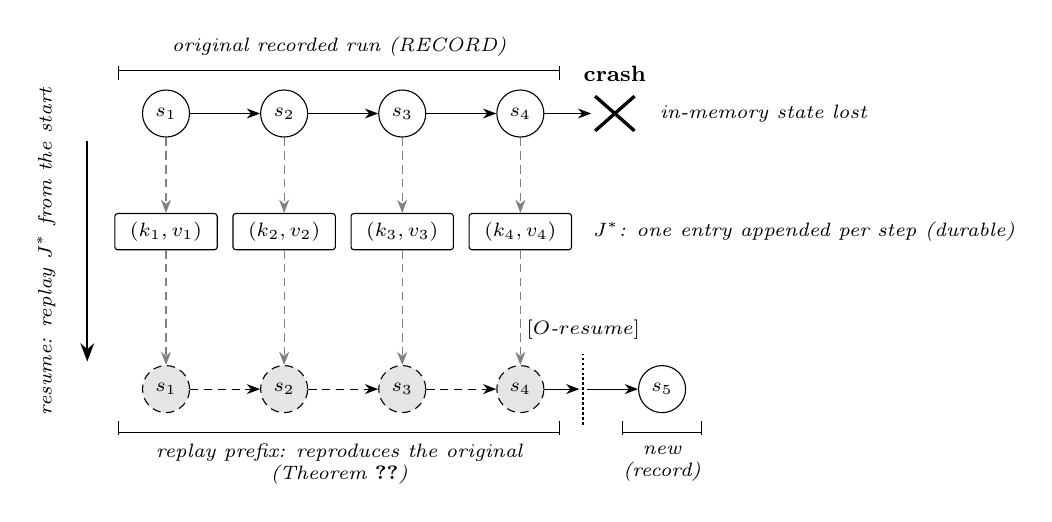
\begin{tikzpicture}[
  >=Stealth,
  every node/.style={align=center, font=\small},
  rec/.style={draw, circle, inner sep=0pt, minimum size=17pt, font=\scriptsize},
  rep/.style={draw, circle, densely dashed, fill=black!10, inner sep=0pt, minimum size=17pt, font=\scriptsize},
  jb/.style={draw, rounded corners=1pt, minimum width=1.3cm, minimum height=0.46cm, inner sep=1pt, font=\scriptsize},
  jv/.style={->, densely dashed, thin, gray},
  lbl/.style={font=\scriptsize\itshape},
]

\foreach \i/\x in {1/2, 2/3.5, 3/5, 4/6.5} { \node[rec] (s\i) at (\x,0) {$s_{\i}$}; }
\draw[->] (s1)--(s2); \draw[->] (s2)--(s3); \draw[->] (s3)--(s4);

\draw[->] (s4) -- (7.4,0);
\draw[very thick] (7.45,-0.22)--(7.95,0.22);
\draw[very thick] (7.95,-0.22)--(7.45,0.22);
\node[font=\footnotesize\bfseries] at (7.7,0.5) {crash};
\node[lbl, anchor=west] at (8.15,0) {in-memory state lost};

\draw[thin] (1.4,0.55)--(7.0,0.55);
\draw[thin] (1.4,0.42)--(1.4,0.6);
\draw[thin] (7.0,0.42)--(7.0,0.6);
\node[lbl] at (4.2,0.85) {original recorded run (RECORD)};

\foreach \i/\x in {1/2, 2/3.5, 3/5, 4/6.5} {
  \node[jb] (j\i) at (\x,-1.5) {$(k_{\i},v_{\i})$};
  \draw[jv] (s\i.south) -- (j\i.north);
}
\node[lbl, anchor=west] at (7.3,-1.5) {$J^*$: one entry appended per step (durable)};

\foreach \i/\x in {1/2, 2/3.5, 3/5, 4/6.5} {
  \node[rep] (r\i) at (\x,-3.5) {$s_{\i}$};
  \draw[jv] (j\i.south) -- (r\i.north);
}
\draw[->, densely dashed] (r1)--(r2);
\draw[->, densely dashed] (r2)--(r3);
\draw[->, densely dashed] (r3)--(r4);

\draw[densely dotted, thick] (7.3,-3.95)--(7.3,-3.05);
\draw[->] (r4) -- (7.25,-3.5);
\node[rec] (s5) at (8.3,-3.5) {$s_5$};
\draw[->] (7.35,-3.5) -- (s5);
\node[lbl] at (7.3,-2.75) {$[O\text{-}resume]$};

\draw[thin] (1.4,-4.05)--(7.0,-4.05);
\draw[thin] (1.4,-3.9)--(1.4,-4.08);
\draw[thin] (7.0,-3.9)--(7.0,-4.08);
\node[lbl, align=center] at (4.2,-4.45) {replay prefix: reproduces the original\\(Theorem~\ref{thm:replay})};
\draw[thin] (7.8,-4.05)--(8.8,-4.05);
\draw[thin] (7.8,-3.9)--(7.8,-4.08);
\draw[thin] (8.8,-3.9)--(8.8,-4.08);
\node[lbl, align=center] at (8.3,-4.45) {new\\(record)};

\draw[->, thick] (1.0,-0.35) -- (1.0,-3.15);
\node[lbl, rotate=90, anchor=south] at (0.72,-1.75) {resume: replay $J^*$ from the start};
\end{tikzpicture}
}
  \caption{Crash recovery (Corollary~\ref{cor:resume}).
    Calls $s_1 \ldots s_4$ run in record mode and append their outcomes to the journal; a crash
    at $s_5$ loses all in-memory state but keeps the journal prefix. Resume replays the prefix
    with probability~1 (\textsc{[O-rep]}), then switches to record mode
    (\textsc{[O-resume]}) for the rest of the run.}
  \label{fig:crash-recovery}
\end{figure}

\subsection{Crash Recovery}

A crash loses the agent's in-memory state but, by (A3), keeps a prefix of the journal.
Recovery resumes the program on that prefix with whatever randomness is available afterwards.
To state the result, define the \emph{splice} of two tapes at cursor $m$ by
\[
  \mathsf{splice}_m(\omega, \omega')(c, p) \;=\;
  \begin{cases}
    \omega(c, p) & c < m,\\
    \omega'(c, p) & c \geq m.
  \end{cases}
\]

\begin{corollary}[Crash recovery]
\label{cor:resume}
For every tree $T$, tapes $\omega$ and $\omega'$, cursor $c$, and $n \in \mathbb{N}$, let $J$
be the journal of $\mathsf{rec}(T, \omega, c)$ and $J_{<n}$ its first $n$ entries.
Then
\[
  \mathsf{res}(T,\; J_{<n},\; \omega',\; c) \;=\; \mathsf{rec}\bigl(T,\; \mathsf{splice}_{c+n}(\omega, \omega'),\; c\bigr).
\]
Consequently:
\begin{enumerate}[label=(\roman*), noitemsep]
  \item \textbf{(Same randomness)} resuming with $\omega' = \omega$ reproduces the uninterrupted
    run exactly, wherever the crash occurred;
  \item \textbf{(Fresh randomness)} if $\omega'$ is drawn from $\mathbb{P}$ independently of
    $\omega$, the resumed run has the same distribution as an uninterrupted record run, and
    conditioned on the surviving prefix $J_{<n}$, its continuation has the same distribution
    as the original run's continuation conditioned on the same prefix.
\end{enumerate}
\end{corollary}

\begin{proof}
The identity is proved by induction on $T$, generalizing over $c$ and $n$, using one auxiliary
fact: a record run from cursor $c$ reads the tape only at cursors $\geq c$, so two tapes that
agree from $c$ on give the same run.
If $n = 0$, resuming on the empty journal is recording on $\omega'$, and
$\mathsf{splice}_c(\omega, \omega')$ agrees with $\omega'$ from $c$ on.
If $n > 0$ and $T = \mathsf{draw}(p, k)$, the first surviving entry is $(c, p, v)$ with
$v = \omega(c, p) = \mathsf{splice}_{c+n}(\omega,\omega')(c, p)$, so both sides make the same
first call and continue with $k(v)$ from cursor $c+1$ with $n-1$ surviving entries, where the
induction hypothesis applies.

For~(i), $\mathsf{splice}_m(\omega, \omega) = \omega$.
For~(ii), the coordinates of $\mathsf{splice}_{c+n}(\omega, \omega')$ are independent with
the right marginals, since those at cursors below $c+n$ come from $\omega$, the rest come from
$\omega'$, and $\omega$ and $\omega'$ are independent; so the spliced tape has law $\mathbb{P}$
and the resumed run has the record distribution.
By Lemma~\ref{lem:cursors} the surviving prefix reads only coordinates at cursors below $c+n$,
on which the two tapes agree, so it is the same random variable under $\omega$ and under the
spliced tape.
The pair (prefix, whole run) therefore has the same joint law under both tapes, and so does the
conditional law of the run given the prefix.
\end{proof}

\begin{remark}[When the crash point is random]
Corollary~\ref{cor:resume} fixes the crash point $n$.
The identity holds for every $n$, so it also holds when $n$ is random.
Part~(ii) then still holds if the crash point is a \emph{stopping time}, meaning whether the
crash happens after $k$ entries depends only on the coordinates at cursors below $c+k$, and is
independent of $\omega'$: replacing the coordinates after a stopping time by independent fresh
ones does not change the law of a tape whose cursor rows are independent and identically
distributed, which is the strong Markov property.
It fails if the crash depends on a response that was drawn but not yet journaled.
For example, let $T$ make one call whose response is a fair coin and return it, and let the
process crash before journaling exactly when the response is $0$.
Then the resumed run returns $1$ with probability $3/4$, not $1/2$.
A recovery guarantee in distribution therefore needs the response to be journaled before
anything that depends on it can crash the agent, which is the order \textsc{[O-rec]} enforces.
\end{remark}

\noindent
For a single agent every prefix of its journal is a valid recovery point, so no
consistent-cut condition is needed; Section~\ref{sec:limitations} explains why concurrent
agents need one.

\subsection{Mechanization}
\label{sec:mechanization}

Lemma~\ref{lem:cursors}, the identity of Theorem~\ref{thm:replay} with part~(i) and the
pointwise core of part~(iii), and the identity of Corollary~\ref{cor:resume} with part~(i) are
mechanized in Lean~4; part~(ii) of the theorem holds by the type of the replay function, which
takes no tape (\texttt{lean/AgenticalT1.lean}, checked with Lean v4.30.0).
The development represents values, prompts, and cursors by natural numbers, programs by the
trees of Section~\ref{sec:syntax}, and tapes by functions
$\mathbb{N} \to \mathbb{N} \to \mathbb{N}$, and quantifies over every tree, tape, starting
cursor, and crash point.
It contains no unproven steps, and \texttt{\#print axioms} reports only Lean's standard axioms
(\texttt{propext}, and \texttt{Quot.sound} for the crash-recovery theorems).
The translation from terms to trees and the measure-theoretic layer, Lemma~\ref{lem:tape} and
the distributional parts of Theorem~\ref{thm:replay}(iii) and Corollary~\ref{cor:resume}(ii),
are on paper; their proofs use the pointwise identities, Lemma~\ref{lem:cursors}, and the
independence and marginals of the tape coordinates.


\section{The Rust Prototype}
\label{sec:rust-runtime}

The \texttt{agentical} Rust crate has no dependencies beyond the standard library.
It defines synchronous, executor-agnostic traits for the agent, the oracle, and the journal,
shown in Listing~\ref{lst:traits}, along with interfaces for channels, memory, and supervision
intended for future multi-agent work (Section~\ref{sec:limitations}).

\begin{lstlisting}[caption={The agent, oracle, and journal traits (doc comments omitted).},label={lst:traits}]
pub trait Agent {
    type State;
    type Out;
    fn step(&mut self, state: &mut Self::State) -> Step<Self::Out>;
}

pub trait Oracle {
    fn sample(&self, prompt: Prompt) -> Sampled;
    fn measure_hint(&self) -> Option<Dist> { None }
}

pub trait Journal {
    fn append(&mut self, agent: &AgentId, event: Event) -> Cursor;
    fn replay_next(&self, agent: &AgentId) -> Outcome;
    fn checkpoint(&self, agent: &AgentId) -> Cursor;
}
\end{lstlisting}

The journal is position-indexed: the cursor is the key, as in Section~\ref{sec:modes}, so there
is no key-to-value map and no collision assumption.
A runtime module implements the semantics for a single agent:
\begin{itemize}[noitemsep]
  \item \texttt{InMemoryJournal}, with \texttt{append}, \texttt{replay\_next}, \texttt{rewind},
    and \texttt{truncate} (to simulate a crash);
  \item \texttt{SeededOracle}, a categorical sampler driven by a SplitMix64 generator, which
    stands in for an LLM;
  \item a driver that runs an agent in record, replay, or resume mode following
    \textsc{[O-rec]}, \textsc{[O-rep]}, and \textsc{[O-resume]}.
\end{itemize}

\paragraph{Side effects.}
The prototype also journals tool side effects, outside the formal results, using a
write-ahead discipline.
Before performing an effect it appends an \emph{intent} record carrying the effect's argument;
after the effect succeeds it appends a \emph{committed} record carrying the result.
Replay returns the journaled result and does not perform the effect again.
A crash between the two records leaves a dangling intent, which recovery detects and resolves
either by performing the effect again with the journaled argument, which is safe for an
idempotent effect of a single agent, or by recording a compensation.
Replaying a compensated effect stops the run without performing anything.
Section~\ref{sec:eval-e2} tests this behaviour at every crash point; formalizing it is future
work.

\paragraph{What is not implemented.}
The channel, memory, and supervisor interfaces have no implementation, so the prototype runs a
single agent.
The journal lives in memory only; there is no persistent backend.


\section{Evaluation}
\label{sec:evaluation}

We evaluate the Rust prototype (Section~\ref{sec:rust-runtime}) on three questions:
does replay reproduce a recorded run (E1), does recovery from a crash at any point preserve
what was journaled and complete the run (E2), and what does journaling cost (E3)?
These experiments test that the implementation follows the record, replay, and resume
semantics for a single agent, matching the scope of the formal results, and they use a seeded
stand-in for the LLM.

\paragraph{Setup.}
The agent is a small loop with two branches.
It draws \texttt{classify} from $\{\texttt{tool}: 5/6,\ \texttt{answer}: 1/6\}$.
On \texttt{tool} it draws \texttt{tool-arg} from $\{\texttt{arg-A}: 3/5,\ \texttt{arg-B}: 2/5\}$
and performs a durable effect \texttt{commit(arg)} under the three-phase write-ahead
discipline; on \texttt{answer} it draws \texttt{answer}, whose distribution has a single
outcome.
A recorded run therefore has two or four journal entries.
The oracle is \texttt{SeededOracle}, a categorical sampler driven by SplitMix64, and the journal
is \texttt{InMemoryJournal}.
All seeds come from a fixed SplitMix64 stream, so every experiment is reproducible.
Measurements were taken on an Apple M5 Pro with 48\,GB of memory, macOS~27.0.1, and
rustc~1.93.0, in release builds.
Each experiment is an integration test in the accompanying repository
(\texttt{tests/eval\_e1.rs}, \texttt{eval\_e2.rs}, \texttt{eval\_e3.rs}) run with \texttt{cargo test --release --test <name> -- --nocapture}.

\subsection{E1: Replay Determinism}
\label{sec:eval-e1}

For each of $N = 1{,}000$ trials we record a run with one seed, then replay the complete
journal with a fresh oracle seeded independently.
We compare the traces (each label carries its journal key and the realized value) and the
final outputs.
Theorem~\ref{thm:replay}(i)--(ii) predicts identical traces in every trial.

\paragraph{Result.}
All $1{,}000$ replays reproduced the recorded trace and output exactly.
Every trial made at least one oracle draw, $810$ took the branch with the durable effect, and
the replay seed differed from the record seed in every trial, so agreement comes from the
journal rather than from the oracle.
Because replay never consults the live oracle, this outcome is expected by construction; the
experiment checks that the implementation conforms to \textsc{[O-rep]} and \textsc{[Eff-rep]}.

\subsection{E2: Crash Recovery at Every Journal Position}
\label{sec:eval-e2}

For each of $1{,}000$ recorded runs, and for every crash point $k$ from $0$ to the journal
length, we keep only the first $k$ journal entries, then resume in replay mode with a fresh
oracle whose seed differs from the recording seed.
If the crash point separates an effect's intent from its committed record, the resumed run
stops at the dangling intent; we then apply Class-I recovery (re-perform with the journaled
argument and commit) and resume again.
For each resume we check that
(a)~the run completes with an output and leaves no dangling intent;
(b)~the first $k$ journal entries are unchanged and every trace label whose entry survived is
reproduced;
(c)~every oracle value lies in the support of its distribution and journal cursors stay dense;
and (d)~an effect whose committed record survived is not performed again.

\paragraph{Result.}
The sweep made $4{,}664$ resumes.
All $4{,}664$ completed and reproduced their surviving prefix, $832$ of them crashed inside an
effect's write-ahead window and were recovered, and no surviving committed effect was performed
again.

\paragraph{Conditional law.}
Corollary~\ref{cor:resume}(ii) says that the resumed continuation follows the original law conditioned on the
replayed prefix.
We check this on the prefix \texttt{classify = tool}: across $20{,}000$ resumes with fresh seeds,
the re-sampled \texttt{tool-arg} was \texttt{arg-A} with frequency $0.5989$, against
$3/5 = 0.6$ (standard error $\approx 0.0035$).

\paragraph{Compensation.}
After a crash inside the write-ahead window followed by a compensating recovery (Class~C),
replaying the journal twice stops both times at the compensated effect, produces no output,
performs no effect, and appends nothing, as the write-ahead design intends.

\paragraph{A defect found by E2.}
An earlier version of the driver stayed in replay mode after \textsc{[O-resume]} fell through to
recording, so the next step re-read the entry just appended as if it were history and could
produce out-of-support values.
The original test suite missed this because its only crash test took the branch whose
distribution has a single outcome; the sweep above fails on that version and passes on the
corrected one.

\subsection{E3: Journaling Overhead}
\label{sec:eval-e3}

\paragraph{Append latency.}
We append $n \in \{10^3, 10^4, 10^5, 10^6\}$ oracle-draw events to an in-memory journal, after
one warm-up pass, and report the mean time per append.
Over six runs, every measurement fell between $88$ and $145$\,ns per append, with no growth in
$n$, consistent with amortized constant-time append; the journal holds exactly one entry per
step.
These are single timed passes per size, not a statistical benchmark.

\paragraph{Replay versus re-execution.}
To model a networked LLM call we inject a latency of $1$\,ms into every oracle draw.
A recorded run then takes about $2.51$\,ms, while replaying it takes $0.5$--$0.8\,\mu$s, a
speedup of about $3{,}200\times$ to $4{,}900\times$ across six runs.
The speedup is dominated by the injected latency: replay performs no oracle calls, so the
time saved per replayed draw is the latency of the call itself.

\paragraph{Not measured.}
We did not measure the cost of journaling relative to a journal-free execution mode, which the
prototype lacks, or the cost of persisting the journal (for example, \texttt{fsync} on every
append), since no persistent backend exists yet.

\subsection{Threats to Validity}
\label{sec:eval-threats}

\paragraph{Internal.}
The seeded oracle stands in for an LLM.
The experiments show that the implementation follows the record/replay semantics, not how real
models behave.
Crashes are simulated by truncating an in-memory journal; torn writes, \texttt{fsync} behavior,
and storage failures are not exercised.

\paragraph{Construct.}
Trace comparison in E1 and E2 uses labels that carry cursors, prompts, and responses, as in
Theorem~\ref{thm:replay}.
E2 checks the conditional law on one prefix and one prompt, not in general.

\paragraph{External.}
All measurements come from one machine and a single in-memory backend, and the workload is a
small agent; results for persistent backends, larger agents, or many concurrent agents may
differ.

\begin{table}[t]
\centering
\caption{Summary of the evaluation.}
\label{tab:eval-summary}
\fitwidth{%
\begin{tabular}{@{}lllp{5.2cm}@{}}
\toprule
\textbf{ID} & \textbf{Question} & \textbf{Result relates to} & \textbf{Outcome} \\
\midrule
E1 & Replay determinism & Theorem~\ref{thm:replay} & $1{,}000/1{,}000$ identical replays \\
E2 & Crash at every position & Corollary~\ref{cor:resume}; side effects & $4{,}664/4{,}664$ resumes correct; no duplicate effects; conditional law matches \\
E3 & Journaling overhead & implementation & 88--145\,ns per append, flat in $n$ \\
\bottomrule
\end{tabular}%
}
\end{table}


\section{Related Work}
\label{sec:related}

\subsection{Formal Models of LLM Agents}

\paragraph{LLMbda and FIDES.}
LLMbda~\citep{garby2026llmbda} is an untyped call-by-value $\lambda$-calculus whose constructs
include prompt-response conversations that can be forked and cleared, code generation, and
dynamic information-flow control in which every value carries a label.
Its first version followed FIDES~\citep{costa2025fides} in assuming that the underlying model is
deterministic; the current version gives a probabilistic semantics, proves a
termination-insensitive probabilistic noninterference theorem for the whole calculus, and uses
its Lean-verified interpreter as the agent harness that calls the model.
FIDES is a planner-based system that enforces information-flow policies around an LLM; its
formal guarantees are stated for a deterministic model function.
Like LLMbda we treat model calls probabilistically, but our main concern is different: LLMbda
studies what an agent's program may do with untrusted data, whereas we study recording,
replaying, and recovering a run. Our noninterference theorem (Theorem~\ref{thm:ni}) addresses
what LLMbda does not model, concurrently scheduled agents, at the price of coarser, per-agent
labels.

\paragraph{Other calculi and languages for agents.}
$\lambda_A$~\citep{liu2026lambdaA} extends the simply typed $\lambda$-calculus with oracle calls,
bounded fixpoints, and probabilistic choice, and proves type safety and termination in Coq.
PPDL~\citep{mandel2026ppdl} treats LLM-based flows as probabilistic programs whose semantics is a
weighted distribution over traces.
Zhou, D'Antoni, and Polikarpova~\citep{zhou2026lbac} have agents generate well-typed Haskell
programs whose information flow is controlled with LIO~\citep{stefan2011lio}, and prove a
soundness theorem with the model treated as a deterministic oracle.
None of these addresses journaling, replay, or crash recovery.

\paragraph{MSC coordination calculus.}
Bollig, F\"{u}gger, and Nowak~\citep{bollig2026msc} specify multi-agent workflows as message
sequence charts in a domain-specific language that separates message-passing structure from
LLM calls, tool calls, and human control points, project global specifications to
deadlock-free local programs, and machine-check all results in Lean~4.
Their implementation, ZipperGen, runs workflows through a persistent store and can replay the
committed history after a restart, although this durability is not part of the formal model.
The calculus establishes coordination properties independently of LLM nondeterminism, treating
model outputs as arbitrary; we instead treat each output as a draw from a measure, which is
what lets us state that replay and recovery preserve distributions.

\paragraph{Other formal and empirical work.}
Schlapbach~\citep{schlapbach2026mcp} gives a process-calculus semantics for agentic tool
protocols such as the Model Context Protocol; the second version of that preprint was withdrawn
because of a logical flaw in one theorem, and a revised version has since been posted.
Zaichyk~\citep{semanticfusion2026} studies decentralized coordination over scoped views of an
ontology-structured shared memory, with probabilistic results about update proposals, and
recovers from failures by re-synchronizing from shared state rather than by replay.
Cemri et al.~\citep{cemri2025mast} build a taxonomy of multi-agent failures from more than
1{,}600 annotated traces.
Khatchadourian~\citep{khatchadourian2026replayable} proposes a protocol for replaying tool-using
financial agents and comparing runs at different levels; it is an empirical harness, not a
semantics.
He and Yu~\citep{he2026postdeterministic} argue, in a short position paper, that systems built
from agents must tolerate divergent execution traces that reach equivalent outcomes.

\subsection{Record, Replay, and Recovery}

\paragraph{Message logging.}
Logging every nondeterministic event so that a process can be replayed after a failure is a
classical technique.
Strom and Yemini's optimistic recovery~\citep{strom1985optimistic} and the message-logging
protocols surveyed by Elnozahy et al.~\citep{elnozahy2002survey} assume that processes are
piecewise deterministic and log the nondeterministic events between deterministic intervals.
Consistent global states are due to Chandy and Lamport~\citep{chandy1985snapshots}, and
compensating transactions to Garcia-Molina and Salem's sagas~\citep{garcia1987sagas}.
Our journal is message logging specialized to an agent whose nondeterministic events are model
calls; what we add is a statement of its soundness inside a probabilistic semantics.

\paragraph{Record, replay, and resume for LLM agents.}
Several recent systems record LLM agent runs at their nondeterministic boundaries and replay
them, for debugging or regression testing~\citep{mudasiru2026agrepl,chawla2026chronicle}.
Khan~\citep{khan2026resume} specifies a checkpoint-and-resume contract for workflow persistence
layers, checks it with machine-checked models, and finds duplicate effects after crashes in
widely used frameworks; Zheng et al.~\citep{zheng2026execedits} give an exact, Lean-mechanized
check of when agent executions can be checkpointed, forked, restored, or merged; and Wu et
al.~\citep{wu2026safetoresume} show that rollback can restore states that are not consistent
causal cuts.
Li~\citep{li2026exactlyonce} proves that no policy based on verification alone achieves
exactly-once effects under late commits without a bound on in-flight time.
These works are deterministic or empirical; ours places replay and recovery inside a
probabilistic semantics, for single agents and for systems under deterministic scheduling.

\paragraph{Durable-execution engines.}
Temporal~\citep{temporal2024docs} re-executes deterministic workflow code against an event
history and records the results of Activities, including LLM calls, and of replay-safe
operations such as random number generation~\citep{temporal2026sideeffects}.
Restate~\citep{restate2026}, DBOS~\citep{dbos2026}, and LangGraph's
checkpointing~\citep{langgraph2026persistence} take related journaling or checkpointing
approaches.
To our knowledge none of these systems comes with a formal semantics in which replay soundness
is a theorem about distributions.

\subsection{Probabilistic Semantics and Guarantees}

Our semantics builds on the sampling view of probabilistic programs~\citep{kozen1981semantics,borgstrom2016probabilistic}
and uses a coupling argument~\citep{barthe2015coupling}.
For LLM agents, Bensalem et al.~\citep{bensalem2026threelayer} argue for chaining probabilistic
assume-guarantee contracts to obtain system-level bounds, and Solko-Breslin et
al.~\citep{solkobreslin2026probverif} bound the probability of policy violations without
independence assumptions; both are complementary to replay, which preserves whatever
probabilities such analyses attach to a run.


\section{Limitations and Future Work}
\label{sec:limitations}

The results of this paper concern a single agent with no recursion and no formalized side
effects.
This section describes the limits of the prototype and what extending the theory requires.
Several of these extensions are subtle: designs that look natural turn out to be unsound, and we
note the pitfalls we know of.

\paragraph{The prototype.}
The oracle in our experiments is a seeded stand-in for an LLM, and the journal is in memory, so
the experiments show that the implementation follows the semantics, not how it behaves with
real models or persistent storage.
Experiments with real LLMs and a journal that survives process crashes are the natural next
step.

\paragraph{Recursion.}
Our terms have no recursion, so every run makes finitely many calls.
Agents that loop until a goal is met need recursion or a bounded loop; the theorems should
extend to finite prefixes of possibly infinite runs, but we have not proved this.

\paragraph{Side effects.}
Write-ahead logging of side effects is implemented and tested but not formalized.
A formal treatment must state what recovery can guarantee.
Performing an interrupted effect again is safe for an idempotent effect of a single agent, but
not in general: if another agent changed the same external state in the meantime, performing
the effect again can undo that change.
Compensation needs its own write-ahead discipline, or a crash during compensation can leave an
effect undone twice or not at all.
Li~\citep{li2026exactlyonce} shows that exactly-once effects cannot be achieved by verification
alone under late commits without a bound on in-flight time, so any recovery theorem must rest on
explicit assumptions about the external system, such as idempotence, atomicity, or a reliable
way to query whether an effect happened.

\paragraph{Concurrent agents.}
With several agents, replay and recovery become substantially harder.
\begin{itemize}[noitemsep]
  \item \emph{Interleaving.} A replayed run must follow the original interleaving of the agents,
    or agents that share state can read different values than they did originally. The
    scheduler's choices must therefore be journaled or reproduced deterministically.
  \item \emph{Recovery points.} Recovery must resume from a consistent cut of the agents'
    journals~\citep{chandy1985snapshots}. With shared memory this must account for which write
    each read observed, not only for messages; Wu et al.~\citep{wu2026safetoresume} show that
    agent frameworks can roll back to states that are not consistent cuts.
  \item \emph{Messages.} Messages sent before a cut but received after it must be delivered
    again exactly once, which requires identifying messages by channel and sequence number
    rather than by value.
  \item \emph{Restart.} Restarting part of a running system, as a supervisor might, also
    requires restoring the restarted agent's local state and suppressing messages it already
    sent.
\end{itemize}

\paragraph{Information-flow control.}
LLMbda~\citep{garby2026llmbda} proves probabilistic noninterference for a single agent's
program.
For concurrently scheduled agents, classical results on multi-threaded programs show that the
scheduler must not observe how long secret computations take, or timing becomes an information
channel~\citep{volpano1999probabilistic,sabelfeld2000probabilistic}.
Coarse-grained floating labels~\citep{stefan2011lio}, as used for agents by
APPA~\citep{kravchenko2026appa}, are a natural discipline, but they must keep the labels of
existing memory cells fixed: if a high-security agent can overwrite a public cell with a
secret label, whether a public agent can later read that cell leaks information.
Parallel composition inside one agent is similarly delicate, because one thread's secret
receive can block another's public output.
Peters-Gill et al.~\citep{petersgill2026camels} show empirically that single-agent defences
against prompt injection do not compose across agents, and Adams~\citep{adams2026sme} obtains
noninterference for language models by running one instance per security level; a
noninterference theorem for concurrently scheduled LLM agents remains open.

\paragraph{Compositional guarantees.}
If each agent of a system meets its own goal with probability at least $p_i$, Boole's
inequality bounds the probability that all do by $1 - \sum_i (1 - p_i)$, without independence.
The hard part is establishing the per-agent bounds inside a system, where an agent's inputs
depend on other agents and on the scheduler; this needs an assume-guarantee argument of the
kind Bensalem et al.~\citep{bensalem2026threelayer} advocate, and complements verification
approaches that bound the probability of violations directly~\citep{solkobreslin2026probverif}.


\section{Conclusion}
\label{sec:conclusion}

We gave a minimal probabilistic semantics for durable replay of an LLM agent, in which every
model call is a draw from an abstract measure and every response is journaled.
In this setting, replaying a run from its journal reproduces it exactly, so record and replay
induce the same distribution over traces, and resuming after a crash continues the run with
the distribution it would have had without the crash, provided the crash does not depend on a
response that was never journaled.
The pointwise core of both results is mechanized in Lean~4, and a Rust prototype that
implements the semantics passes replay and crash-recovery tests at every journal position.
The results place a classical recovery technique, logging nondeterministic events, inside a
probabilistic semantics, so durability no longer requires treating each model call as an opaque
value with no distribution.
Both results extend to systems of concurrent agents under deterministic scheduling with a
single global journal, and such systems satisfy a probabilistic noninterference theorem under a
floating-label discipline with fixed labels on memory and channels and a priority scheduler
whose priorities depend only on public events.
Distributed journals, formalized side effects, finer-grained information flow, and
mechanizing the noninterference proof are the main directions for future work.


\section*{Acknowledgments and Use of AI Tools}
\addcontentsline{toc}{section}{Acknowledgments and Use of AI Tools}
I developed this work with Anthropic's Claude as a collaborator on the proofs, code, and
writing. Any errors are my own.

\bibliographystyle{plainnat}
\bibliography{refs}

\end{document}
